% mnras_template.tex 
%
% LaTeX template for creating an MNRAS paper
%
% v3.0 released 14 May 2015
% (version numbers match those of mnras.cls)
%
% Copyright (C) Royal Astronomical Society 2015
% Authors:
% Keith T. Smith (Royal Astronomical Society)

% Change log
%
% v3.0 May 2015
%    Renamed to match the new package name
%    Version number matches mnras.cls
%    A few minor tweaks to wording
% v1.0 September 2013
%    Beta testing only - never publicly released
%    First version: a simple (ish) template for creating an MNRAS paper

%%%%%%%%%%%%%%%%%%%%%%%%%%%%%%%%%%%%%%%%%%%%%%%%%%
% Basic setup. Most papers should leave these options alone.
\documentclass[fleqn,usenatbib]{mnras}

% MNRAS is set in Times font. If you don't have this installed (most LaTeX
% installations will be fine) or prefer the old Computer Modern fonts, comment
% out the following line
\usepackage{newtxtext,newtxmath}
% Depending on your LaTeX fonts installation, you might get better results with one of these:
%\usepackage{mathptmx}
%\usepackage{txfonts}

% Use vector fonts, so it zooms properly in on-screen viewing software
% Don't change these lines unless you know what you are doing
\usepackage[T1]{fontenc}

% Allow "Thomas van Noord" and "Simon de Laguarde" and alike to be sorted by "N" and "L" etc. in the bibliography.
% Write the name in the bibliography as "\VAN{Noord}{Van}{van} Noord, Thomas"
\DeclareRobustCommand{\VAN}[3]{#2}
\let\VANthebibliography\thebibliography
\def\thebibliography{\DeclareRobustCommand{\VAN}[3]{##3}\VANthebibliography}


%%%%% AUTHORS - PLACE YOUR OWN PACKAGES HERE %%%%%

% Only include extra packages if you really need them. Common packages are:
\usepackage{graphicx}	% Including figure files
\usepackage{amsmath}	% Advanced maths commands
%\usepackage{amssymb}	% Extra maths symbols
\usepackage{comment}
%%%%%%%%%%%%%%%%%%%%%%%%%%%%%%%%%%%%%%%%%%%%%%%%%%

%%%%% AUTHORS - PLACE YOUR OWN COMMANDS HERE %%%%%

% Please keep new commands to a minimum, and use \newcommand not \def to avoid
% overwriting existing commands. Example:
\newcommand{\swiftj}{SWIFT J1749.4-2807}
\newcommand{\nicer}{NICER}
\newcommand{\xmm}{XMM-Newton}

	% per cm-squared

%%%%%%%%%%%%%%%%%%%%%%%%%%%%%%%%%%%%%%%%%%%%%%%%%%

%%%%%%%%%%%%%%%%%%% TITLE PAGE %%%%%%%%%%%%%%%%%%%

% Title of the paper, and the short title which is used in the headers.
% Keep the title short and informative.
\title[Short title, max. 45 characters]{SWIFT J1749.4-2807}

% The list of authors, and the short list which is used in the headers.
% If you need two or more lines of authors, add an extra line using \newauthor
\author[Sanna et al.]{
A. Sanna,$^{1}$\thanks{E-mail: andrea.sanna@dsf.unica.it}
$^{2}$
$^{2,3}$
$^{3}$
\\
% List of institutions
$^{1}$Dipartimento di Fisica, Università degli Studi di Cagliari, SP Monserrato-Sestu km 0.7, 09042 Monserrato, Italy\\
$^{2}$\\
$^{3}$
}

% These dates will be filled out by the publisher
\date{Accepted XXX. Received YYY; in original form ZZZ}

% Enter the current year, for the copyright statements etc.
\pubyear{2015}

% Don't change these lines
\begin{document}
\label{firstpage}
\pagerange{\pageref{firstpage}--\pageref{lastpage}}
\maketitle

% Abstract of the paper
\begin{abstract}
It should be a single paragraph not more than 250 words (200 words for Letters).
\end{abstract}

% Select between one and six entries from the list of approved keywords.
% Don't make up new ones.
\begin{keywords}
binaries:general–stars:neutron – X-rays:binaries – accretion: accretion disks
\end{keywords}

%%%%%%%%%%%%%%%%%%%%%%%%%%%%%%%%%%%%%%%%%%%%%%%%%%

%%%%%%%%%%%%%%%%% BODY OF PAPER %%%%%%%%%%%%%%%%%%

\section{Introduction}


\section{Observations and data reduction}

Normally the next section describes the techniques the authors used.
It is frequently split into subsections, such as Section~\ref{sec:maths} below.

\subsection{NICER}
%\label{sec:maths} % used for referring to this section from elsewhere

NICER \citep{Gendreau:2012vf} started observing the X-ray transient \swiftj{} on 2021 March 1 (MJD 59274.6) up to 2021 March 28 (MJD 59301.8) for a total exposure time of almost 141~ks. We processed the NICER observations with the NICERDAS pipeline version 7.0 (version V007a) retaining events in the 0.2–12 keV energy range, for which the pointing offset was <54 arcsec, the dark Earth limb angle was $>30^\circ$, the bright Earth limb angle was $>40^\circ$, and the ISS location was outside of the South Atlantic Anomaly (SAA). Morepver, we selected events fromt 52 out of the avaibale 56 aligned pairs of X-ray concentrator optics and silicon drift detectors (\textbf{Check with Keith}).



%\begin{equation}
%    x=\frac{-b\pm\sqrt{b^2-4ac}}{2a}.
%	\label{eq:quadratic}
%\end{equation}


\subsection{XMM-Newton}

XMM-Newton \citep{Jansen2001} triggered a target of opportunity observation of \swiftj{} (Obs. ID. 0872392001) starting from 2021 March 4 at 08:41 UTC and ending on 2021 March 4 at 16:17 UTC, for a total durantion of 56.7 ks. 
The instrumental set-up during the observation included the Epic-pn (PN) camera operated in timing mode, the Epic-MOS 1–2 in small window and timing mode, respectively, while the RGS in spectroscopy mode. For the poirpouse of this work we focused on the PN observation only. We extracted the PN dataset using the Science Analysis Software (SAS) v.19 with up-to-date calibration files. We retained events in the energy range 0.5–10 keV, by selecting optimally calibrated events with \textsc{PATTERN $\leq$ 4} and \textsc{(FLAG = 0)}. We filtered source and background events from the PN instrument within the RAWX regions [29:47] and [2:8], respectively. We investigated for possible high background flaring activity by constructing a 20s resolution light-curve of the source event at energies larger than 10 keV, but we found none.  
The 0.5-10 keV light-curve of the source shows an average count-rate around 40 counts per seconds. Superimposed are clearly visible six type-I X-ray bursts almost evenly spaced with a recurrence time of 2.2 hours, and two full X-ray eclipses. 


\subsection{NuSTAR}

\section{Data analysis and results}
%\subsection{Timing analysis}

Both NICER and XMM-Newton observations registered several X-ray type-I bursts and X-ray eclipses during the outburst of the source. To investigate the temporal behavious of the X-ray pulsar we decided to exclude them from the analaysis by ignoring time intervals of $\pm 50$ seconds before and after the events. Moreover, we retained only events with energies within the range 0.5 to 10 keV. We then corrected the photon arrival times to the solar system barycenter using the Chandra coordinates of the source \citep{Jonker:2013wp}.


Starting from the timing solution obtained for the first outburst of the source \citep{Markwardt:2010tl}, we applyed baricentric correction to the photon time of arrivals of the \nicer{} and \xmm{} datasets to account for the Doppler effect in the binary system assuming a circular orbit \citep[see e.g.][for a detailed description of the method]{Burderi:2007tl,Sanna:2016ty}. Following on the prelimary detection of the X-ray pulsation during the 2021 outburst of the source \citep{Bult:2021wk}, we updated the time of passage from the ascending node ($T_{ASC}$) to be able to recover the coherent signal. Before applying phase coherent timing analysis, we refined the values of the local $T_{ASC}$ and the mean spin frequency. We explored the local $T_{ASC}$ value by sampling the interval $59274.49427\pm P_{orb}/2$ at 1 second steps. For each $T_{ASC}$ value we corrected the applyed baricentric correction keeping the other orbital parameters fixed. We then applyied epoch-folding searching techniques of the whole dataset using 16 phase bins by exploring the frequency space around the value reported by \citet{Bult:2021wk} with steps of $10^{-8}$ Hz for a total of 10001 steps. Under the assumption that the best orbital solution is represented by the folded pulse profile at largest $\chi^2$ value in the epoch-folding search \citep[see
e.g.][]{Kirsch:2004tg}, we obtained $T_{ASC}=59274.49428$ MJD and $\overline{\nu}=517.92001388$.
It is worth noting that the estimated local $T_{ASC}$ value significantly differs from the predicted value obtained by propagating the orbital solution reported by \citep{Markwardt:2010tl} assuming a constant orbital period. As it will be discussed in detial in the next sections, the latter result suggests the presence of a signifincant evolution of the orbital period of the system.

To perform coherent timing analysis, we applied the updated local timing solution to created 8-phase-bin pulse profiles by epoch-folding 2000 s-long data segments at the mean spin frequency $\overline{\nu}$. If required, we adjusted the length of the data segments in order to improve the significance of the pulse profiles. We modelled the pulse profiles by fitting a costant plus a superposition of two harmonically related sinuoidal components. We retained only harmonics for which the ratio between the sinusoidal amplitude and the corresponding $1\sigma$ uncertainty is equal or grater than three. For each significant component we inferred the fractional amplitude defined as the ratio between the sinusoidal amplitude and the soure photons collected to crate the pulse profile (i.e. total number of photons in the profile minus the corresponding background) and the fractional part of the phase residual. Higher harmonics were not required to describe the pulse profile.

The second panel of Fig.~\ref{fig:phase_fit} shows the evolution of the background corrected fractional amplitude of the fundamental (solid squares) and second harmonic (empty circles) components of the \nicer{} (black points) and \xmm{} (red points) datasets during the outburst. Upper limits (triangles) at $3\sigma$ conidence lever are reported for the time intervals in which no significant detection was available.  


We modelled the fundamental and second harmonic components describing the pulse profiles of the source by applying standard timing techniques \citep[see e.g.][for more details]{Burderi:2007tl, Sanna:2018wh}. More specifically, we modelled the phase temporal evolution as:
\begin{equation}
\Delta \phi(t)= \phi_0 - \Delta \nu_0(t-T_0)- \frac{1}{2} \dot{\nu}(t-T_0)^2+R_{orb}(t),
\end{equation}
whith $\phi_0$, $\Delta \nu_0$ and $\dot{\nu}$ representing a constant phase, the correction factor on the frequency used to epoch-fold the data, and the spin frequency derivative referred to the epoch $T_0$. $R_{orb}(t)$ describes the residual orbital modulation arising from differential corrections between the guessed NS ephemeris and the real one \citep[see e.g.][]{Deeter:1981te}.

We iteratively repeated this process for each refined ephemeris until no significant improvements were found for any of the model parameters. In Table~\ref{tab:sol} we list the   the orbital best-fit parameters as well as the spin frequency parameters obtained independently from the analysis of the fundamental and second harmonic components. In the third and fourth pannels of Fig.~\ref{fig:phase_fit} we show the phase delay residuals with the best-fitting models for the fundamental and and second harmonic, respectively. 

\begin{table*}

\begin{tabular}{l | c  c  }
\hline
Parameters             & Fundamental & Second Harmonic\\
\hline
\hline
R.A. (J2000) &  \multicolumn{2}{c}{$17^h49^m31^s.73\pm0.6^s$}\\
Decl. (J2000) & \multicolumn{2}{c}{$-28^\circ08'05''.08\pm0.6''$} \\
Orbital period $P_{orb}$ (s) & 31740.84(1) & 31740.8417(27)\\
Projected semi-major axis $a \sin i/c$ (lt-s) & 1.89956(3) &1.899568(11) \\
Ascending node passage $T_{\text{NOD}}$ (MJD) & 59274.494176(5) & 59274.4941787(14)\\
Eccentricity ($e$) & $3.7(3.3)\times 10^{-5}$ &$4.1(1.1)\times 10^{-5}$\\
$\chi^2$/d.o.f. &1001.6/84 & 97.8/60\\
\hline
\hline
Spin frequency $\nu_0$ (Hz) &517.92001572(25)$^*$& 517.92001385(16)$^*$\\
Spin frequency 1st derivative $\dot{\nu}_0$ (Hz/s) &-4.0(5)$\times 10^{-12}$$^*$&$-0.6(1.1)\times 10^{-13}$$^*$\\
\hline
\end{tabular}
\caption{Timing solution obtained from the analysis of the \nicer{} and \xmm{} observations collected during the whole 2021 outburst of \swiftj{} . The orbital solution is referred to the epoch T$_0$=59274.6 MJD. Errors are at 1$\sigma$ confidence level.$^*$ Uncertainties have been calculated including the contribution of the positional uncertainties.}
\label{tab:solution}
\end{table*}

To take into account the values of $\tilde{\chi}^2>1$, we rescaled the uncertainties on the parameters reported in Tab.~\ref{tab:solution} by a factor $\sqrt{\chi^2}$ \citep[see e.g.][]{Finger:1999vb}.

We investigated the contribution of the positional uncertainties on the spin frequency and its derivative by considering the residuals induced by the Earth's motion assuming small variations of the source position $\delta_{\lambda}$ and $\delta_{\gamma}$ (ecliptic coordinates) expressed by the relation:
\begin{equation}
R_{pos}(t) = - \nu_0 y [\sin(M_0+\epsilon)\cos \gamma \delta\lambda -  \cos(M_0+\epsilon)\sin \gamma \delta\gamma],
\label{eq:pos}
\end{equation}
where $y=r_E/c$ represents the Earth semi-major axis in light-seconds, $M_0=2 \pi (T_0-T_{v})/P_{\oplus}-\lambda$, $T_{v}$ and $P_{\oplus}$ are the vernal point and the Earth orbital period, respectively, and $\epsilon=2\pi(t-T_0)/P_{\oplus}$ \citep[see, e.g.][]{Lyne90}. Given the short duration of the outburst with respect to Earth's orbital period, we can solve Eq.\ref{eq:pos} by expanding it in series of $\epsilon\ll1$ \cite[see e.g.][and references therein]{Burderi:2007tl}. This allows to estimate upper limits on the spin frequency correction and the spin derivative as $\sigma_{\nu_{pos}}\leq \nu_0y\sigma_{v}(1+\sin^2\gamma)^{1/2}2\pi/P_{\oplus}$ and $\sigma_{\dot{\nu}_{pos}}\leq \nu_0y\sigma_{v}(1+\sin^2\gamma)^{1/2}(2\pi/P_{\oplus})^2$, respectively, where $\sigma_{v}$ represents the positional error circle. Using the source position reported in Tab.~\ref{tab:solution} \citep{Jonker:2013wp}, we estimated $\sigma_{\nu_{pos}} \leq 1.4\times 10^{-7}$ Hz and $\sigma_{\dot{\nu}_{pos}} \leq 3\times 10^{-14}$ Hz/s, respectively. We added in quadrature these systematic uncertainties to the statistical errors of $\nu_0$ and $\dot{\nu}$ estimated from the timing analysis.


\begin{comment}
\textbf{to be updated}
\end{comment}
The average pulse profile differs significantly from a sinusoidal function. It is well described by using a combination of two sinusoids shifted in phase. The XMM-Newton (NuSTAR) fundamental and second harmonic have background-corrected fractional amplitudes of 5.6\% (4\%) and 3.4\% (1.6\%), respectively. For the NICER average profile we obtain fractional ampli- tudes of 4.7\% and 3.1\% for the fundamental and second harmonic (not corrected for the background), respectively.

\begin{figure*}
\centering
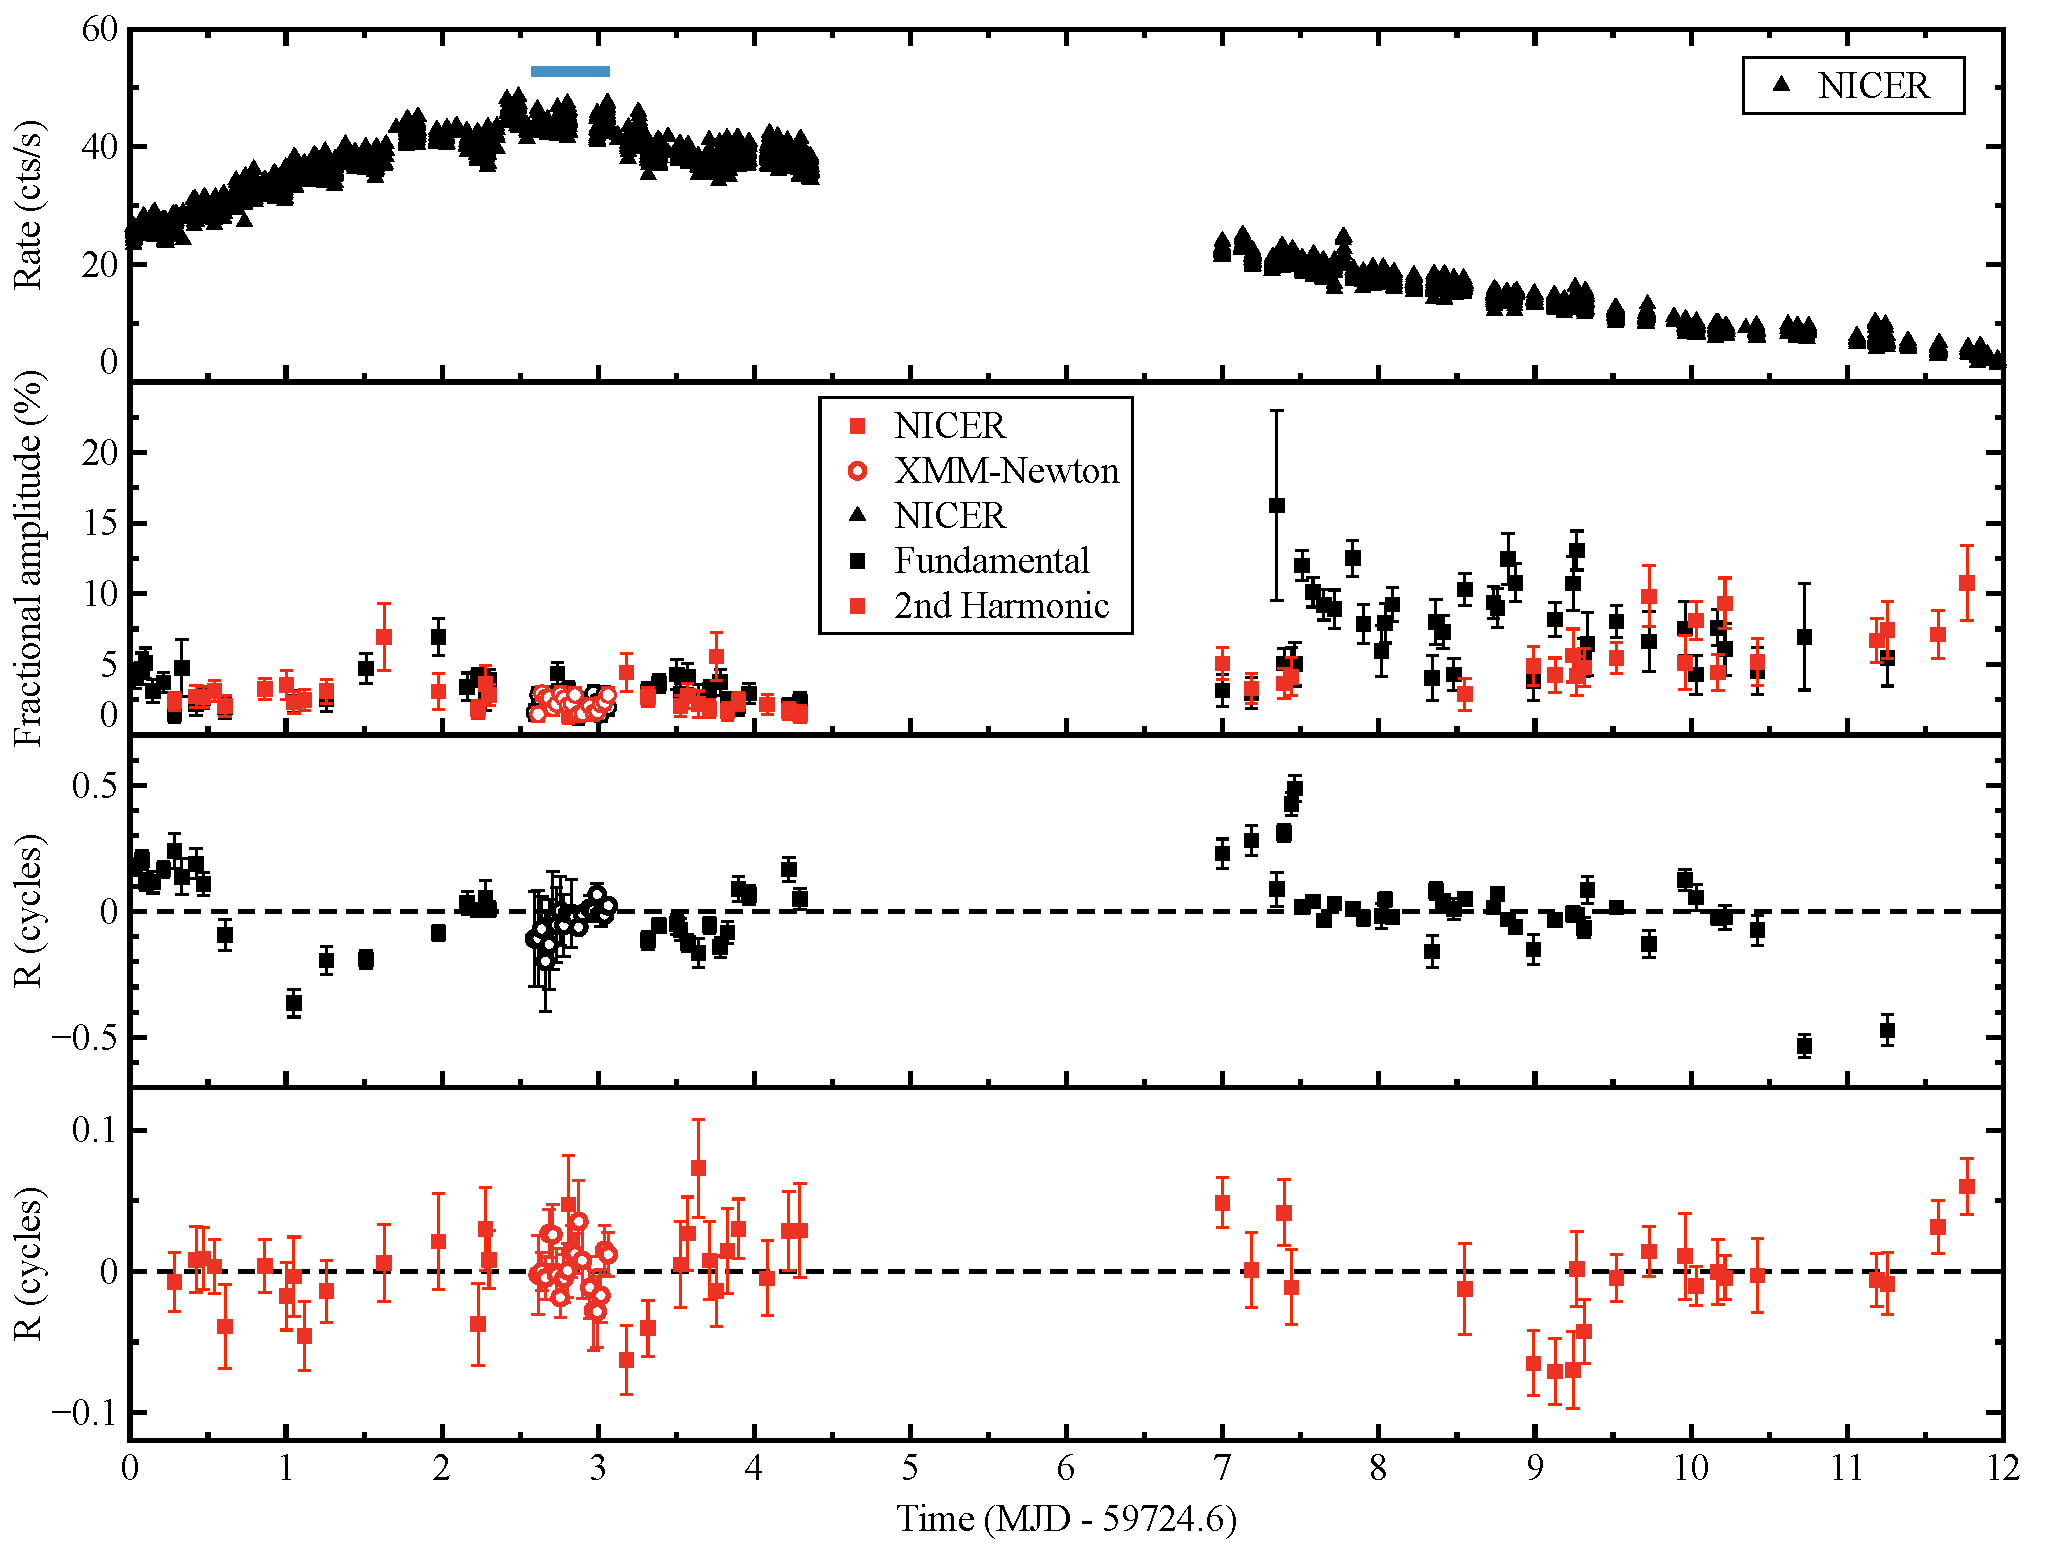
\includegraphics[width=0.8\textwidth]{plot_lc_phase_residuals}
\caption{\textit{First panel -} \nicer{} 0.5-10 keV light-curve of the 2021 outburst of the accreting millisecond X-ray pulsar \swiftj{}. The blue segment identifies the time interval in which the \xmm{} observation has been performed. \textit{Second panel -} Time evolution of the fractional amplitude determined for the fundamental (black points) and the second harmonic (red points) components used to model the source pulse profiles created from the \nicer{} (filled squares) and \xmm{} (empty circles) datasets. \textit{Third panel -} Fundamental pulse phase residuals in units of phase cycles relative to the best-fitting solution. \textit{Fourth panel -} Second harmonic pulse phase residuals in units of phase cycles relative to the best-fitting solution.}
\label{fig:phase_fit}
\end{figure*} 


% Example table
%\begin{table}
%	\centering
%	\caption{This is an example table. Captions appear above each table.
%	Remember to define the quantities, symbols and units used.}
%	\label{tab:example_table}
%	\begin{tabular}{lccr} % four columns, alignment for each
%		\hline
%		A & B & C & D\\
%		\hline
%		1 & 2 & 3 & 4\\
%		2 & 4 & 6 & 8\\
%		3 & 5 & 7 & 9\\
%		\hline
%	\end{tabular}
%\end{table}


%\section{Results}


Finally, by combining the more accurate orbital ephemerides reported for the 2010 outburst of the source \citep{Markwardt:2010tl}, we investigated the long term orbital evolution by studying independently the variation of the orbital period and the delay accumulated by $T_{NOD}$ as a function the orbital cycles elapsed since its discovery. 

The variation of the orbital period obtained by combining the most accurate timing solution of the last two outbursts of \swiftj{} is $\Delta P_{orb}=0.1227(84)$ s. Interestingly and not commonly reported for AMXPs, the secular obital evoliution can be directly estimated by the direct measument of the orbital period thanks to its relative large variation and the small uncertainties associated with the single measurments \citep[somehting similar has been observed only for the AMXP IGR J17511-3057][]{Riggio2021}. Taking into account that the number of orbital cycles elapsed in between the two outbursts is $N=10817$, we can estimate an orbital peridod derivative $\dot{P}_{orb}=3.6(2)\times 10^{-10}$ s/s compatible with a fast expansion of the binary system.

The presence of significant first derivative of the orbital period of the system should affect the evolution of other orbital parameters such as the time of passage from the ascending node. In fact, by extending the analogy of coherent timing analysis to the orbital parametes, we can approximate $T_{NOD}$ with the expression

\begin{equation}
\label{eq:evo}
T_{NOD}=T_{0,NOD}+N P_{0,orb}+\frac{1}{2}N^2P_{0,orb}\dot{P}_{orb},
\end{equation}
where $T_{0,NOD}$, $P_{0,orb}$ and $\dot{P}_{orb}$ represent the time of passage from the ascending node, the orbital period and its derivativs with respect to a specific reference epoch, respectively. 
To verify the compatibility of the $T_{NOD}$ values mesured in the two outbursts with the inferred orbital period derivative, we take the 2010 orbital solution as a reference and we estimated the $T_{NOD}$ value for the latest outburst assuming $\dot{P}_{orb}=3.6(2)\times 10^{-10}$ s/s. To be able to use Eq.\ref{eq:evo}, we quantify the number of orbital cycles elapsed in between the two outbursts as N=INT[($T_{2021,NOD}-T_{2010,NOD}$/$P_{2010,orb}$], where INT represents the closest integer. Combining all we estimate a guess of the time of passage from the ascenfing node of $T_{2021,NOD}=59274.4950(14)$ MJD, which is compatible within uncertaities with the measured value reported in the Table.\ref{tab:solution}.



\section{Discussion}

\begin{itemize}
We have reported an updated timing solution for the perculiar accreting millisecond X-ray pulsar \swiftj{} obtained by performing phase-coherent timing analysis of the X-ray pulsations detected by \nicer{} and \xmm{} during the latest outburst of the source. Interestingly, the new set of orbital parameters show significant signs of temporal evolution with respect to the timing solution obtained from the first outburst \citep{Markwardt:2010tl}, which likely suggests conspicuous mass-loss from the companion star. Moreover, we find evidence of low eccentricy 
	
\item \textbf{Jumps in the fundamental component: pulse profile changes?}
\item \textbf{maybe creation of pulse profiles at different times during the outburst}





\item \textbf{comparison with 2010 solution}
\item \textbf{Asin(i)/c expansion marginally significant if we take all errors into account. Expansion is too fast, it would require to much matter lost - Apply Kepler's third law logaritmic derivative to show that}
\item \textbf{Eccentricity larger than 0, marginally significant but in line with 2010. Possible to exoplain with Phynney 1982. - Verify whether the same values are found also in binary radio millisecond pulsars}
\item \textbf{Orbital period expansion - discuss possible scenarios of mass transferr}
\item \textbf{Long-term spin frequency evolution - I need to correct for the new coordinates}
\item \textbf{...}
\end{itemize}

\subsection{Orbital evolution}

\section*{Acknowledgements}





%%%%%%%%%%%%%%%%%%%% REFERENCES %%%%%%%%%%%%%%%%%%

% The best way to enter references is to use BibTeX:

\bibliographystyle{mnras}
\bibliography{/Users/asanna/Desktop/Work/biblio.bib} % if your bibtex file is called example.bib


% Alternatively you could enter them by hand, like this:
% This method is tedious and prone to error if you have lots of references
%\begin{thebibliography}{99}
%\bibitem[\protect\citeauthoryear{Author}{2012}]{Author2012}
%Author A.~N., 2013, Journal of Improbable Astronomy, 1, 1
%\bibitem[\protect\citeauthoryear{Others}{2013}]{Others2013}
%Others S., 2012, Journal of Interesting Stuff, 17, 198
%\end{thebibliography}

%%%%%%%%%%%%%%%%%%%%%%%%%%%%%%%%%%%%%%%%%%%%%%%%%%

%%%%%%%%%%%%%%%%% APPENDICES %%%%%%%%%%%%%%%%%%%%%

%\appendix

%\section{Some extra material}


%%%%%%%%%%%%%%%%%%%%%%%%%%%%%%%%%%%%%%%%%%%%%%%%%%


% Don't change these lines
\bsp	% typesetting comment
\label{lastpage}
\end{document}

% End of mnras_template.tex
